\section{Introduction}
\label{sec:intro} 

The inference of emotions through expressions has been a topic of interest for the past years as it might give insights into a person's feelings towards other individuals or topics. Mehrabian and Wiener~\cite{mehrabian1967decoding} suggest 55\% of communication is perceived by expressions. Lapakko~\cite{Lapakko2015CommunicationI9} argues, however, that these findings are limited to emotional states. Automation of analysis of expressions to get insights into user experience is one step towards live feedback without direct interaction with an individual. 

\begin{figure}[t]
    \centering
    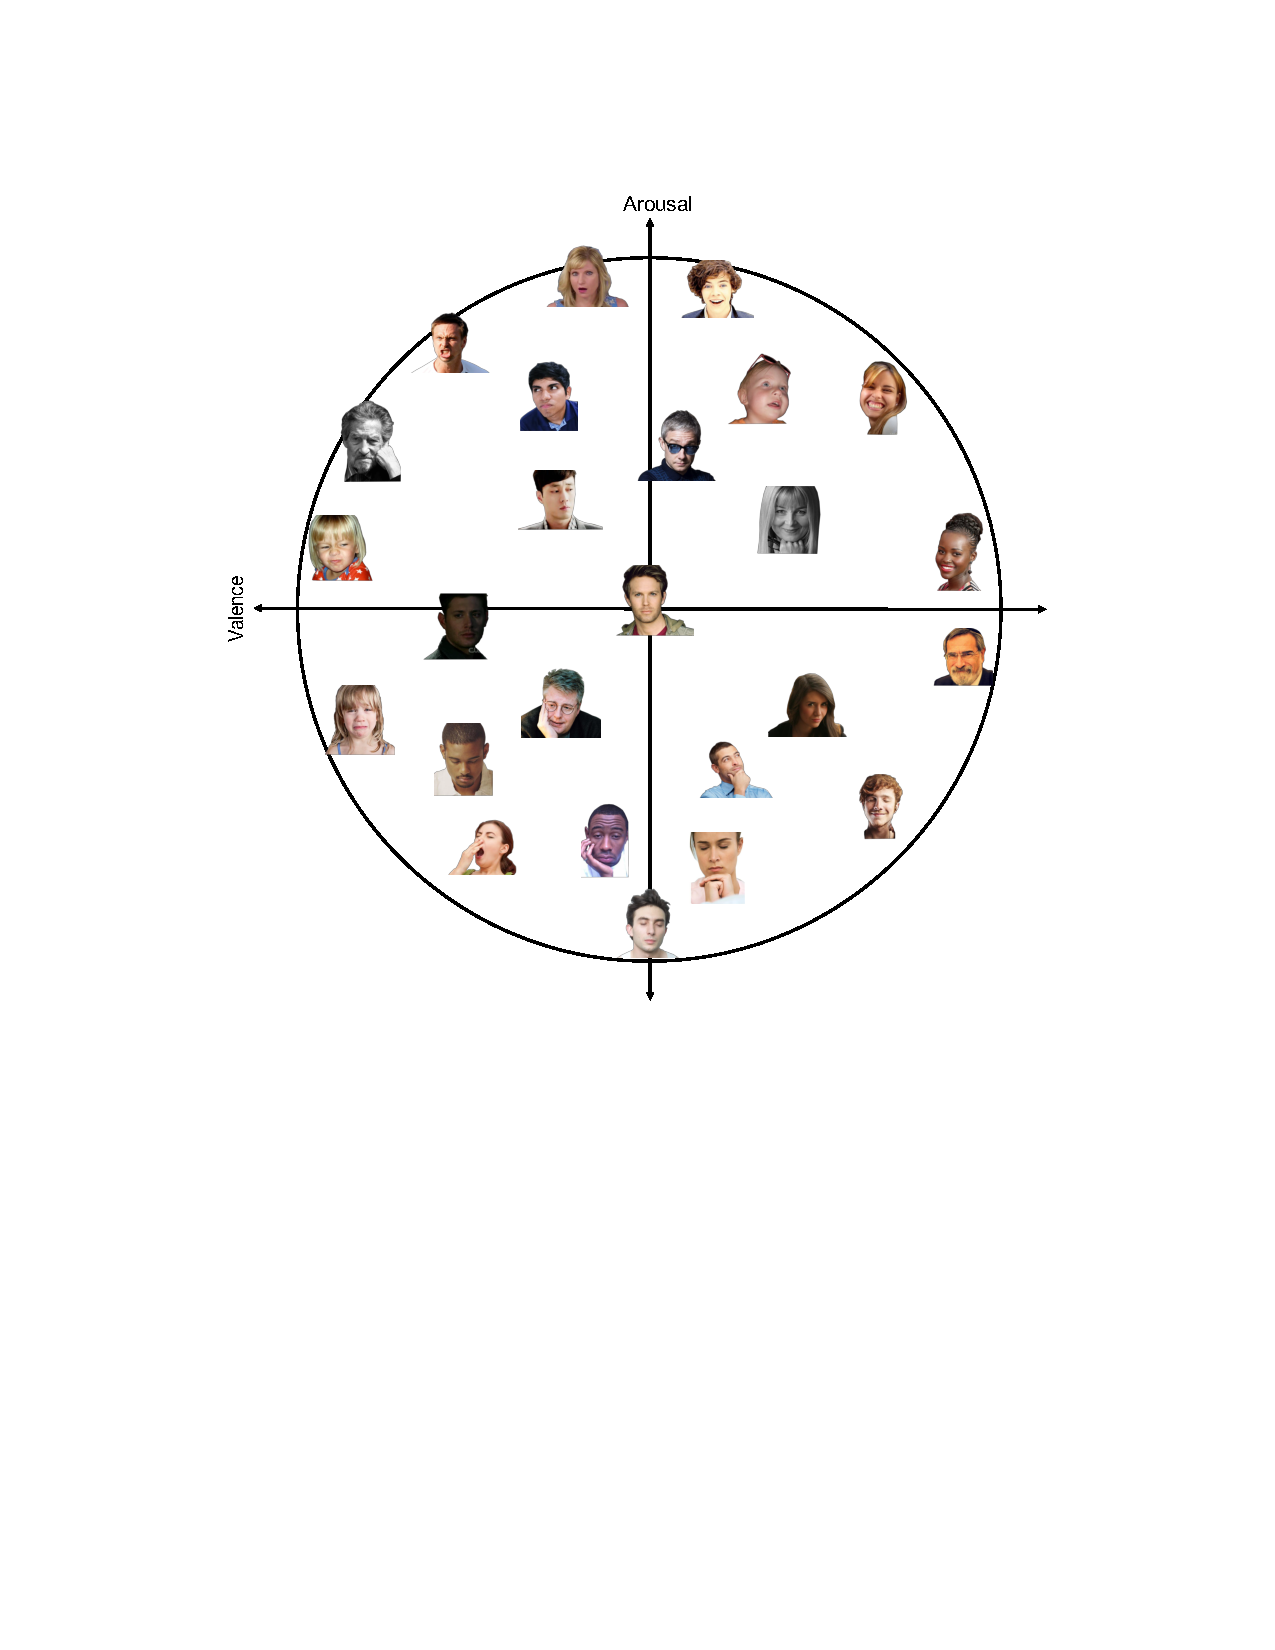
\includegraphics[width=0.8\columnwidth, trim={3cm 11cm 3cm 3cm}, clip]{pictures/affectnet/Bild_Russel_AffectNet.pdf}
    \caption{\textit{Valence/arousal} for sample images from \affectnet{}~\cite{mollahosseini2017affectnet}.}
    \label{fig:Russel_Affectnet}
\end{figure}


A common approach is \textit{expression inference}, i.e. classification of emotional expressions into discrete categories. However, a comprehensive meta-analysis of facial expressions research by Barrett et al.~\cite{barretetal2019}  has shown, that there is no consensus across cultures and intra-cultural over specific facial movements reliably depicting one category of emotion. They suggest that affective states can more reliably be inferred by a third-party individual. They emphasize that these states are inferred, not recognized. According to Russell~\cite{rusellmodell}, affects can be described as a set of dimensions with each dimension varying independently. These dimensions are called \va{}, representing the positivity/negativity and intensity-/activation of expressions respectively. Using \va{} of the circumplex model of affect~\cite{rusellmodell} as additional dimensions rather than only discrete emotions for expression inference thus offers a more robust framework, as they provide a continuous spectrum that captures the underlying affective states.


In this work, we compare training with \va{} labels merged with the commonly used discrete emotions to train with the two approaches separately. 
Our approach involves pinpointing the differences and similarities between two leading datasets that catalog images according to their explicit discrete and continuous emotional states: \affectnet~\cite{mollahosseini2017affectnet} and \emotic{}~\cite{kosti_emotic_2017}. 
% We examine the labeling process and show that there is still a need for further datasets to create a universal model that does not guess emotions based on labels of third-party individuals but rather gets information about the true internal state of each image subject.
% We refer to~\cite{barretetal2019} for a more detailed discussion. 
We then develop a lightweight deep neural network tailored for computer vision tasks, aiming to accurately infer these discrete emotions as well as the continuous dimensions of \va{}, surpassing the performance of existing models. In particular, our model improves accuracy by reducing the root-mean-square error  (RMSE) by 7.0\% for \val{} and 6.8\% for \aro{}. It also increases the concordance correlation coefficients (CCC) by 0.8\% for \val{} and 2.0\% for \aro{} when tested on the \affectnet{} dataset. These improvements are reflected in our final results, with CCC values of 0.716 for \val{} and 0.642 for \aro{}, and RMSE values of 0.331 for \val{} and 0.305 for \aro{}. Furthermore, we exceed the top-3 accuracy set by Khan \etal~\cite{khan2024focusclip} on the \emotic{} dataset by 1.0\%. %Additionally, we conduct a cross-evaluation of the model's effectiveness using the given test datasets. %In summary, this research focuses on the following question:
% Consequently, the impact of these approaches needs to be measured. To do so, we 
% \begin{enumerate} [label=(\roman*)]
%     \item identify differences and similarities of two state-of-the-art datasets containing images with their apparent discrete and continuous emotion states
%     \item enhance a lightweight deep neural network architecture suited for computer vision to suggest these discrete emotions and/or continuous dimensions \va{}l{}, \aro{}
%     \item cross-evaluate the resulting model performances on the given test datasets. Hence, the following research question motivates our research:
% \end{enumerate}
%\textit{What effect does the addition of \val{}/\aro{} regression to discrete emotion classification have on facial emotion guessing performance across datasets?} 

%In the following we examine related work in \autoref{sec:relatedwork}, looking into different datasets and related approaches in emotion guessing. Then, we describe our applied data analysis and our model training approach in \autoref{sec:method}. Subsequently, we share our insights on the data and the outcomes of our model training in \autoref{sec:results}. Lastly, we present our conclusions and future perspectives in \autoref{sec:conclusion}.
